\subsection{Controller design (Mikkel)}

Since the program has several different components that must communicate, it was important for us to have these communications centralized as much as possible. This resulted in having three controllers throughout the program. These correspond to the three main parts, namely the user interface, the internal logic and the database. Since we have a singular controller for each of these, it is very easy to extend the functionality of the program as a whole. 

% Needs more.... very not finished

\begin{figure}[H]
\centering
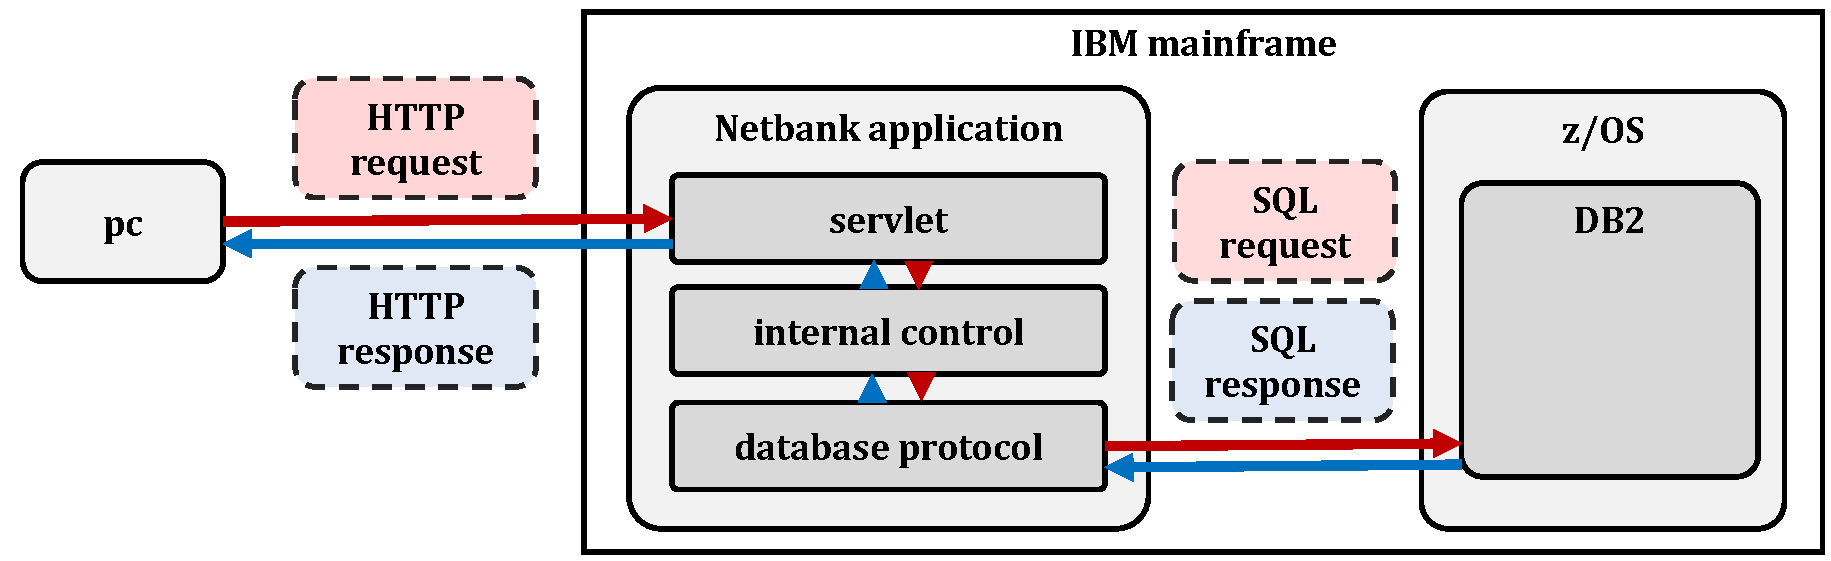
\includegraphics[width = 0.9\textwidth]{figures/control_flow.pdf}
\caption{Control flow in the program, and how the three controllers interact with the program.}
\label{fig:designcontrol}
\end{figure}